% Options for packages loaded elsewhere
\PassOptionsToPackage{unicode}{hyperref}
\PassOptionsToPackage{hyphens}{url}
%
\documentclass[
]{article}
\usepackage{amsmath,amssymb}
\usepackage{lmodern}
\usepackage{iftex}
\ifPDFTeX
  \usepackage[T1]{fontenc}
  \usepackage[utf8]{inputenc}
  \usepackage{textcomp} % provide euro and other symbols
\else % if luatex or xetex
  \usepackage{unicode-math}
  \defaultfontfeatures{Scale=MatchLowercase}
  \defaultfontfeatures[\rmfamily]{Ligatures=TeX,Scale=1}
\fi
% Use upquote if available, for straight quotes in verbatim environments
\IfFileExists{upquote.sty}{\usepackage{upquote}}{}
\IfFileExists{microtype.sty}{% use microtype if available
  \usepackage[]{microtype}
  \UseMicrotypeSet[protrusion]{basicmath} % disable protrusion for tt fonts
}{}
\makeatletter
\@ifundefined{KOMAClassName}{% if non-KOMA class
  \IfFileExists{parskip.sty}{%
    \usepackage{parskip}
  }{% else
    \setlength{\parindent}{0pt}
    \setlength{\parskip}{6pt plus 2pt minus 1pt}}
}{% if KOMA class
  \KOMAoptions{parskip=half}}
\makeatother
\usepackage{xcolor}
\usepackage[margin=1in]{geometry}
\usepackage{color}
\usepackage{fancyvrb}
\newcommand{\VerbBar}{|}
\newcommand{\VERB}{\Verb[commandchars=\\\{\}]}
\DefineVerbatimEnvironment{Highlighting}{Verbatim}{commandchars=\\\{\}}
% Add ',fontsize=\small' for more characters per line
\usepackage{framed}
\definecolor{shadecolor}{RGB}{248,248,248}
\newenvironment{Shaded}{\begin{snugshade}}{\end{snugshade}}
\newcommand{\AlertTok}[1]{\textcolor[rgb]{0.94,0.16,0.16}{#1}}
\newcommand{\AnnotationTok}[1]{\textcolor[rgb]{0.56,0.35,0.01}{\textbf{\textit{#1}}}}
\newcommand{\AttributeTok}[1]{\textcolor[rgb]{0.77,0.63,0.00}{#1}}
\newcommand{\BaseNTok}[1]{\textcolor[rgb]{0.00,0.00,0.81}{#1}}
\newcommand{\BuiltInTok}[1]{#1}
\newcommand{\CharTok}[1]{\textcolor[rgb]{0.31,0.60,0.02}{#1}}
\newcommand{\CommentTok}[1]{\textcolor[rgb]{0.56,0.35,0.01}{\textit{#1}}}
\newcommand{\CommentVarTok}[1]{\textcolor[rgb]{0.56,0.35,0.01}{\textbf{\textit{#1}}}}
\newcommand{\ConstantTok}[1]{\textcolor[rgb]{0.00,0.00,0.00}{#1}}
\newcommand{\ControlFlowTok}[1]{\textcolor[rgb]{0.13,0.29,0.53}{\textbf{#1}}}
\newcommand{\DataTypeTok}[1]{\textcolor[rgb]{0.13,0.29,0.53}{#1}}
\newcommand{\DecValTok}[1]{\textcolor[rgb]{0.00,0.00,0.81}{#1}}
\newcommand{\DocumentationTok}[1]{\textcolor[rgb]{0.56,0.35,0.01}{\textbf{\textit{#1}}}}
\newcommand{\ErrorTok}[1]{\textcolor[rgb]{0.64,0.00,0.00}{\textbf{#1}}}
\newcommand{\ExtensionTok}[1]{#1}
\newcommand{\FloatTok}[1]{\textcolor[rgb]{0.00,0.00,0.81}{#1}}
\newcommand{\FunctionTok}[1]{\textcolor[rgb]{0.00,0.00,0.00}{#1}}
\newcommand{\ImportTok}[1]{#1}
\newcommand{\InformationTok}[1]{\textcolor[rgb]{0.56,0.35,0.01}{\textbf{\textit{#1}}}}
\newcommand{\KeywordTok}[1]{\textcolor[rgb]{0.13,0.29,0.53}{\textbf{#1}}}
\newcommand{\NormalTok}[1]{#1}
\newcommand{\OperatorTok}[1]{\textcolor[rgb]{0.81,0.36,0.00}{\textbf{#1}}}
\newcommand{\OtherTok}[1]{\textcolor[rgb]{0.56,0.35,0.01}{#1}}
\newcommand{\PreprocessorTok}[1]{\textcolor[rgb]{0.56,0.35,0.01}{\textit{#1}}}
\newcommand{\RegionMarkerTok}[1]{#1}
\newcommand{\SpecialCharTok}[1]{\textcolor[rgb]{0.00,0.00,0.00}{#1}}
\newcommand{\SpecialStringTok}[1]{\textcolor[rgb]{0.31,0.60,0.02}{#1}}
\newcommand{\StringTok}[1]{\textcolor[rgb]{0.31,0.60,0.02}{#1}}
\newcommand{\VariableTok}[1]{\textcolor[rgb]{0.00,0.00,0.00}{#1}}
\newcommand{\VerbatimStringTok}[1]{\textcolor[rgb]{0.31,0.60,0.02}{#1}}
\newcommand{\WarningTok}[1]{\textcolor[rgb]{0.56,0.35,0.01}{\textbf{\textit{#1}}}}
\usepackage{graphicx}
\makeatletter
\def\maxwidth{\ifdim\Gin@nat@width>\linewidth\linewidth\else\Gin@nat@width\fi}
\def\maxheight{\ifdim\Gin@nat@height>\textheight\textheight\else\Gin@nat@height\fi}
\makeatother
% Scale images if necessary, so that they will not overflow the page
% margins by default, and it is still possible to overwrite the defaults
% using explicit options in \includegraphics[width, height, ...]{}
\setkeys{Gin}{width=\maxwidth,height=\maxheight,keepaspectratio}
% Set default figure placement to htbp
\makeatletter
\def\fps@figure{htbp}
\makeatother
\setlength{\emergencystretch}{3em} % prevent overfull lines
\providecommand{\tightlist}{%
  \setlength{\itemsep}{0pt}\setlength{\parskip}{0pt}}
\setcounter{secnumdepth}{-\maxdimen} % remove section numbering

\usepackage{amsmath}
\usepackage{xcolor}
\usepackage{graphicx}

%%%%%%%%%%%%% defining colors
\definecolor{navyblue}{RGB}{18, 97, 158}

\usepackage{caption}
\usepackage{fancyhdr}
\usepackage[document]{ragged2e}
\pagestyle{fancy}

%%%%%%%%%%%%%%%%%%%%%%%%%%%%%%%%%%%%%%%%%%%%%%%%%%%%%%%%%
%%%%%% MODIFIER ICI
%%%%%%%%%%%%%%%%%%%%%%%%%%%%%%%%%%%%%%%%%%%%%%%%%%%
\fancyfoot[L]{Équipe 09} % NUMÉRO D'ÉQUIPE
\fancyfoot[R]{ACT-4114} % SIGLE DU COURS
\fancyfoot[C]{\thepage}

\setlength{\headheight}{12.80502pt}

\renewcommand{\contentsname}{Table des Matières}
\newcommand{\bcenter}{\begin{center}}
\newcommand{\ecenter}{\end{center}}
\ifLuaTeX
  \usepackage{selnolig}  % disable illegal ligatures
\fi
\IfFileExists{bookmark.sty}{\usepackage{bookmark}}{\usepackage{hyperref}}
\IfFileExists{xurl.sty}{\usepackage{xurl}}{} % add URL line breaks if available
\urlstyle{same} % disable monospaced font for URLs
\hypersetup{
  hidelinks,
  pdfcreator={LaTeX via pandoc}}

\author{}
\date{\vspace{-2.5em}}

\begin{document}

%\documentclass[12pt]{article}
%\usepackage[english]{babel}
%\usepackage[utf8x]{inputenc}
%\usepackage{amsmath}
%\usepackage{graphicx}
%\usepackage[colorinlistoftodos]{todonotes}
%
%\begin{document}

\begin{titlepage}

\newcommand{\HRule}{\rule{\linewidth}{0.5mm}} % Defines a new command for the horizontal lines, change thickness here
%%% MODIFIER ICI (iNFORMATION GÉNÉRALE DU TRAVAIL)%%%%%%%%%%%%%%%%%%%%%%%%%%%%%%%%%%%%%%%%%%%%%%%

\center % Center everything on the page
\textsc{\LARGE Premier rapport}\\[1.0cm] % LAISSER TP OU METTRE UN VRAI TITRE
\textsc{\Large Apprentissage statistique en actuariat}\\[0.2cm] % NOM DU COURS 
\textsc{\large ACT-4114}\\[0.7cm] % SIGLE
\textsc{\large Équipe 09}\\[0.7cm] % ÉQUIPE

%%%%%%%%%%%%%%%%%%%%%%%%%%%%%%%%%%%%%%%%%%%%%%%%%%%%%%%%%%%%%%%%%%%%%
%%% MODIFIER ICI (TITRE DU TRAVAIL)
%%%%%%%%%%%%%%%%%%%%%%%%%%%%%%%%%%%%%%%%%%%%%%%%%%%%%%%%%%%%%%%%%%%%%

\HRule \\[0.4cm]
{ \Large \bfseries Rapport}\\[0.20cm] { \huge \bfseries Nom de votre TP}\\[0.20cm]

\HRule \\[2cm]
%%% MODIFIER ICI (nOM DES ÉTUDIANTS)%%%%%%%%%%%%%%%%%%%%%%%%%%%%%%%%%%%%%%%%%%%%%%%
\begin{minipage}{0.4\textwidth}
    \begin{flushleft} \large
    \emph{Par}\\
        Danny \textsc{Larochelle}\\
        Maryjane \textsc{Bastille}\\
        Isabelle \textsc{Legendre}\\
        Henri \textsc{Lebel}\\
        Félix-Antoine \textsc{Paris}
    \end{flushleft}
\end{minipage}
~%%% MODIFIER ICI (NI DES ÉTUDIANTS)%%%%%%%%%%%%%%%%%%%%%%%%%%%%%%%%%%%%%%%%%%%%%%%
\begin{minipage}{0.4\textwidth}
    \begin{flushright} \large
    \emph{Numéro d'identification}\\
        111 174 586\\
        111 268 504\\
        536 768 666\\
        111 286 185\\
        536 776 223
    \end{flushright}
\end{minipage} \\[1.0cm]
%%% MODIFIER ICI (NOM DU/DE LA PROF)%%%%%%%%%%%%%%%%%%%%%%%%%%%%%%%%%%%%%%%%%%%%%%%
\emph{Travail présenté à} \\
\emph{Monsieur} \\[0.1cm]
\textsc{\Large Olivier \textsc{Côté}\\[1.0cm]
%%% MODIFIER ICI (DATE)%%%%%%%%%%%%%%%%%%%%%%%%%%%%%%%%%%%%%%%%%%%%%%%
\textsc{\large 13 mars 2023}\\[1cm] % Date, change the \today to a set date if you want to be precise


\includegraphics[width = 10cm]{ul-actuariat}\\[1.5cm]
 
\vfill % Fill the rest of the page with whitespace

\end{titlepage}
%\end{document}

\centering

\clearpage

\tableofcontents

\justify  
\clearpage

\hypertarget{introduction}{%
\section{Introduction}\label{introduction}}

\hypertarget{analyse-exploratoire-des-donnuxe9es}{%
\section{Analyse exploratoire des
données}\label{analyse-exploratoire-des-donnuxe9es}}

\hypertarget{suxe9lection-des-variables}{%
\subsection{Sélection des variables}\label{suxe9lection-des-variables}}

La première étape du travail a consisté à réduire la dimension du jeu de
données. En effet, celui-ci est constitué de 41 variables, dont une
bonne partie n'étant pas utiles dans le contecte de l'analyse des
montants de réclamation. \newline \newline Sans effectuer aucune analyse
statistique, nous avons jugé adéquat de retirer plusieurs variables du
modèle, notamment, toutes les variables contenant beaucoup de valeurs
manquantes, comme baseFloodElevation, basementEnclosureCrawlspace,
elevationCertificateIndicator, elevationDifference, rateMethod et
lowestAdjacentGrade. Ces variables sont aussi toutes issues de
l'évaluation de quelques uns des bâtiments assurés, alors que plusieurs
autres variables telles que numberOfFloorsInTheInsuredBuilding,
originalConstructionDate ou encore lowestFloorElevation auront un impact
probablement plus marqué sur le modèle sans devoir nécessiter un travail
ardu et approximatif d'estimation d'une grande quantité de données
manquantes. \newline \newline Nous avons aussi pris la décision
d'enlever les variables temporelles à l'exception de la date de
construction du bâtiment (originalConstructionDate) et la date du
sinistre (dateOfLoss), puisqu'elles sont les seules variables
temporelles pertinentes à notre analyse selon nous. \newline \newline On
observe aussi que les variables

\hypertarget{cruxe9ation-de-la-nouvelle-variable-ruxe9ponse}{%
\subsection{Création de la nouvelle variable
réponse}\label{cruxe9ation-de-la-nouvelle-variable-ruxe9ponse}}

Dans le jeu de données se retrouvent trois colonnes contenant des
informations sur les montants de prestations payés en lien avec le
bâtiment (amountPaidOnBuildingClaim), les biens
(amountPaidOnContentsClaim) et l'augmentation des coûts en lien avec la
conformité (amountPaidOnIncreasedCostOfComplianceClaim).

\begin{Shaded}
\begin{Highlighting}[]
\NormalTok{data.raw }\OtherTok{\textless{}{-}} \FunctionTok{read.csv}\NormalTok{(}\StringTok{"Flood\_California.csv"}\NormalTok{)}
\end{Highlighting}
\end{Shaded}

\begin{Shaded}
\begin{Highlighting}[]
\DocumentationTok{\#\# Retirer les variables inutiles}
\NormalTok{data.rm }\OtherTok{\textless{}{-}}\NormalTok{ data.raw[, }\FunctionTok{c}\NormalTok{(}\DecValTok{1}\NormalTok{, }\DecValTok{3}\NormalTok{, }\DecValTok{4}\NormalTok{, }\DecValTok{5}\NormalTok{, }\DecValTok{6}\NormalTok{, }\DecValTok{13}\NormalTok{, }\DecValTok{14}\NormalTok{, }\DecValTok{15}\NormalTok{, }\DecValTok{16}\NormalTok{, }\DecValTok{21}\NormalTok{, }\DecValTok{25}\NormalTok{, }\DecValTok{27}\NormalTok{, }\DecValTok{28}\NormalTok{, }\DecValTok{33}\NormalTok{, }\DecValTok{39}\NormalTok{, }\DecValTok{41}\NormalTok{)]}
\NormalTok{data }\OtherTok{\textless{}{-}}\NormalTok{ data.raw[, }\SpecialCharTok{{-}}\FunctionTok{c}\NormalTok{(}\DecValTok{1}\NormalTok{, }\DecValTok{3}\NormalTok{, }\DecValTok{4}\NormalTok{, }\DecValTok{5}\NormalTok{, }\DecValTok{6}\NormalTok{, }\DecValTok{13}\NormalTok{, }\DecValTok{14}\NormalTok{, }\DecValTok{15}\NormalTok{, }\DecValTok{16}\NormalTok{, }\DecValTok{21}\NormalTok{, }\DecValTok{25}\NormalTok{, }\DecValTok{27}\NormalTok{, }\DecValTok{28}\NormalTok{, }\DecValTok{33}\NormalTok{, }\DecValTok{39}\NormalTok{, }\DecValTok{41}\NormalTok{)]}

\CommentTok{\# Combiner les variables réponses (totalAmount)}
\NormalTok{data}\SpecialCharTok{$}\NormalTok{amountPaidOnBuildingClaim[}\FunctionTok{is.na}\NormalTok{(data}\SpecialCharTok{$}\NormalTok{amountPaidOnBuildingClaim)] }\OtherTok{\textless{}{-}} \DecValTok{0}
\NormalTok{data}\SpecialCharTok{$}\NormalTok{amountPaidOnBuildingClaim }\OtherTok{\textless{}{-}}
  \FunctionTok{abs}\NormalTok{(data}\SpecialCharTok{$}\NormalTok{amountPaidOnBuildingClaim)}
\NormalTok{data}\SpecialCharTok{$}\NormalTok{amountPaidOnContentsClaim[}\FunctionTok{is.na}\NormalTok{(data}\SpecialCharTok{$}\NormalTok{amountPaidOnContentsClaim)] }\OtherTok{\textless{}{-}}\DecValTok{0}
\NormalTok{data}\SpecialCharTok{$}\NormalTok{amountPaidOnContentsClaim }\OtherTok{\textless{}{-}}
  \FunctionTok{abs}\NormalTok{(data}\SpecialCharTok{$}\NormalTok{amountPaidOnContentsClaim)}
\NormalTok{data}\SpecialCharTok{$}\NormalTok{amountPaidOnIncreasedCostOfComplianceClaim[}\FunctionTok{is.na}\NormalTok{(data}\SpecialCharTok{$}\NormalTok{amountPaidOnIncreasedCostOfComplianceClaim)] }\OtherTok{\textless{}{-}} \DecValTok{0}
\NormalTok{data}\SpecialCharTok{$}\NormalTok{amountPaidOnIncreasedCostOfComplianceClaim }\OtherTok{\textless{}{-}}
  \FunctionTok{abs}\NormalTok{(data}\SpecialCharTok{$}\NormalTok{amountPaidOnIncreasedCostOfComplianceClaim)}
\NormalTok{data}\SpecialCharTok{$}\NormalTok{totalAmount }\OtherTok{\textless{}{-}} \FunctionTok{apply}\NormalTok{(data[, }\DecValTok{17}\SpecialCharTok{:}\DecValTok{19}\NormalTok{], }\DecValTok{1}\NormalTok{, sum)}
\NormalTok{data }\OtherTok{\textless{}{-}}\NormalTok{ data[, }\SpecialCharTok{{-}}\FunctionTok{c}\NormalTok{(}\DecValTok{17}\NormalTok{, }\DecValTok{18}\NormalTok{, }\DecValTok{19}\NormalTok{)]}

\CommentTok{\# Retirer les lignes n\textquotesingle{}étant pas localisées en Californie}
\NormalTok{data }\OtherTok{\textless{}{-}}\NormalTok{ data[}\SpecialCharTok{!}\FunctionTok{is.na}\NormalTok{(data}\SpecialCharTok{$}\NormalTok{longitude),]}
\NormalTok{data }\OtherTok{\textless{}{-}}\NormalTok{ data[data}\SpecialCharTok{$}\NormalTok{longitude }\SpecialCharTok{\textless{}=} \SpecialCharTok{{-}}\DecValTok{110}\NormalTok{,]}

\CommentTok{\# Imputation par régression linéaire des codes de régions (countyCode)}
\NormalTok{mod.county }\OtherTok{\textless{}{-}} \FunctionTok{lm}\NormalTok{(countyCode }\SpecialCharTok{\textasciitilde{}}\NormalTok{ latitude }\SpecialCharTok{+}\NormalTok{ longitude, }\AttributeTok{data =}\NormalTok{ data)}
\NormalTok{pred.county }\OtherTok{\textless{}{-}} \FunctionTok{predict}\NormalTok{(mod.county, }\AttributeTok{newdata =}\NormalTok{ data[}\FunctionTok{is.na}\NormalTok{(data}\SpecialCharTok{$}\NormalTok{countyCode),], }\AttributeTok{type =} \StringTok{"response"}\NormalTok{)}
\NormalTok{data}\SpecialCharTok{$}\NormalTok{countyCode[}\FunctionTok{is.na}\NormalTok{(data}\SpecialCharTok{$}\NormalTok{countyCode)] }\OtherTok{\textless{}{-}}\NormalTok{ pred.county}
\NormalTok{data }\OtherTok{\textless{}{-}}\NormalTok{ data[data}\SpecialCharTok{$}\NormalTok{countyCode }\SpecialCharTok{!=} \DecValTok{32031}\NormalTok{,]}

\CommentTok{\# Attribution de la classe 10 aux données manquantes de la variable communityRatingSystemDiscount (Les valeurs manquantes sont dans des zones qui ne participent pas au système de rabais, et la classe 10 indique les zones n\textquotesingle{}ayant pas droit à un rabais.)}

\NormalTok{data}\SpecialCharTok{$}\NormalTok{communityRatingSystemDiscount[}\FunctionTok{is.na}\NormalTok{(data}\SpecialCharTok{$}\NormalTok{communityRatingSystemDiscount)] }\OtherTok{\textless{}{-}} \DecValTok{10}

\CommentTok{\# Reclassifiaction de la variable occupancyType}
\NormalTok{data}\SpecialCharTok{$}\NormalTok{occupancyType }\OtherTok{\textless{}{-}} \FunctionTok{as.factor}\NormalTok{(data}\SpecialCharTok{$}\NormalTok{occupancyType)}
\FunctionTok{levels}\NormalTok{(data}\SpecialCharTok{$}\NormalTok{occupancyType) }\OtherTok{\textless{}{-}} \FunctionTok{c}\NormalTok{(}\StringTok{"1"}\NormalTok{, }\StringTok{"2"}\NormalTok{, }\StringTok{"2"}\NormalTok{, }\StringTok{"3"}\NormalTok{, }\StringTok{"1"}\NormalTok{, }\StringTok{"1"}\NormalTok{, }\StringTok{"2"}\NormalTok{, }\StringTok{"2"}\NormalTok{, }\StringTok{"1"}\NormalTok{, }\StringTok{"2"}\NormalTok{, }\StringTok{"2"}\NormalTok{, }\StringTok{"3"}\NormalTok{, }\StringTok{"3"}\NormalTok{, }\StringTok{"3"}\NormalTok{)}

\CommentTok{\# Niveau 1: Résidences familiales}
\CommentTok{\# Niveau 2: Copropriétés résidentielles}
\CommentTok{\# Niveau 3: Non{-}résidentiel}

\CommentTok{\# Attribution de la classe 6 de la variable occupancy à la classe 2 selon la proportion initiale des données dans la classe 6 ressemblant à ceux de la classe 1 (6 n\textquotesingle{}étant pas dans la description des classes par FEMA)}

\CommentTok{\# Éliminaion des données manquant la variable occupancyType}
\NormalTok{data }\OtherTok{\textless{}{-}}\NormalTok{ data[}\SpecialCharTok{{-}}\FunctionTok{which}\NormalTok{(}\FunctionTok{is.na}\NormalTok{(data}\SpecialCharTok{$}\NormalTok{occupancyType)),]}

\CommentTok{\# Imputation des données manquantes de la variable numberOfFloorsInTheInsuredBuilding de facon aléatoire selon la proportion de la variable occupancyType de type 1}

\NormalTok{prop.occ1 }\OtherTok{\textless{}{-}} \FunctionTok{cumsum}\NormalTok{(}\FunctionTok{prop.table}\NormalTok{(}\FunctionTok{table}\NormalTok{(data}\SpecialCharTok{$}\NormalTok{numberOfFloorsInTheInsuredBuilding[}\FunctionTok{which}\NormalTok{(data}\SpecialCharTok{$}\NormalTok{occupancyType }\SpecialCharTok{==} \DecValTok{1}\NormalTok{)])))}


\NormalTok{imp.occ1 }\OtherTok{\textless{}{-}}\NormalTok{ data}\SpecialCharTok{$}\NormalTok{numberOfFloorsInTheInsuredBuilding[}\FunctionTok{which}\NormalTok{(}\FunctionTok{is.na}\NormalTok{(data}\SpecialCharTok{$}\NormalTok{numberOfFloorsInTheInsuredBuilding))]}
\FunctionTok{set.seed}\NormalTok{(}\DecValTok{6969}\NormalTok{)}
\NormalTok{RNG }\OtherTok{\textless{}{-}} \FunctionTok{runif}\NormalTok{(}\FunctionTok{length}\NormalTok{(imp.occ1))}
\ControlFlowTok{for}\NormalTok{(i }\ControlFlowTok{in} \DecValTok{1}\SpecialCharTok{:}\FunctionTok{length}\NormalTok{(imp.occ1))\{}
  \ControlFlowTok{if}\NormalTok{(RNG[}\DecValTok{1}\NormalTok{] }\SpecialCharTok{\textless{}=}\NormalTok{ prop.occ1[}\DecValTok{1}\NormalTok{])}
\NormalTok{    imp.occ1[i] }\OtherTok{\textless{}{-}} \DecValTok{1}
\ControlFlowTok{if}\NormalTok{(RNG[i] }\SpecialCharTok{\textgreater{}}\NormalTok{ prop.occ1[}\DecValTok{1}\NormalTok{] }\SpecialCharTok{\&}\NormalTok{ RNG[i] }\SpecialCharTok{\textless{}=}\NormalTok{ prop.occ1[}\DecValTok{2}\NormalTok{])}
\NormalTok{    imp.occ1[i] }\OtherTok{\textless{}{-}} \DecValTok{2}
  \ControlFlowTok{if}\NormalTok{(RNG[i] }\SpecialCharTok{\textgreater{}}\NormalTok{ prop.occ1[}\DecValTok{2}\NormalTok{] }\SpecialCharTok{\&}\NormalTok{ RNG[i] }\SpecialCharTok{\textless{}=}\NormalTok{ prop.occ1[}\DecValTok{3}\NormalTok{])}
\NormalTok{    imp.occ1[i] }\OtherTok{\textless{}{-}} \DecValTok{3}
\ControlFlowTok{if}\NormalTok{(RNG[i] }\SpecialCharTok{\textgreater{}}\NormalTok{ prop.occ1[}\DecValTok{3}\NormalTok{] }\SpecialCharTok{\&}\NormalTok{ RNG[i] }\SpecialCharTok{\textless{}=}\NormalTok{ prop.occ1[}\DecValTok{4}\NormalTok{])}
\NormalTok{    imp.occ1[i] }\OtherTok{\textless{}{-}} \DecValTok{4}
  \ControlFlowTok{if}\NormalTok{(RNG[i] }\SpecialCharTok{\textgreater{}}\NormalTok{ prop.occ1[}\DecValTok{4}\NormalTok{] }\SpecialCharTok{\&}\NormalTok{ RNG[i] }\SpecialCharTok{\textless{}=}\NormalTok{ prop.occ1[}\DecValTok{5}\NormalTok{])}
\NormalTok{    imp.occ1[i] }\OtherTok{\textless{}{-}} \DecValTok{5}
  \ControlFlowTok{if}\NormalTok{(RNG[i] }\SpecialCharTok{\textgreater{}}\NormalTok{ prop.occ1[}\DecValTok{5}\NormalTok{])}
\NormalTok{    imp.occ1[i] }\OtherTok{\textless{}{-}} \DecValTok{6}
\NormalTok{\}}

\NormalTok{data}\SpecialCharTok{$}\NormalTok{numberOfFloorsInTheInsuredBuilding[}\FunctionTok{which}\NormalTok{(}\FunctionTok{is.na}\NormalTok{(data}\SpecialCharTok{$}\NormalTok{numberOfFloorsInTheInsuredBuilding))] }\OtherTok{\textless{}{-}}\NormalTok{ imp.occ1}


\CommentTok{\# Changement du type de variable pour les dates}
\NormalTok{data}\SpecialCharTok{$}\NormalTok{dateOfLoss }\OtherTok{\textless{}{-}} \FunctionTok{as.Date}\NormalTok{(data}\SpecialCharTok{$}\NormalTok{dateOfLoss)}

\FunctionTok{sum}\NormalTok{(}\FunctionTok{format}\NormalTok{(data}\SpecialCharTok{$}\NormalTok{dateOfLoss, }\StringTok{"\%Y"}\NormalTok{) }\SpecialCharTok{!=}\NormalTok{ data}\SpecialCharTok{$}\NormalTok{yearOfLoss)}
\end{Highlighting}
\end{Shaded}

\begin{verbatim}
## [1] 0
\end{verbatim}

\begin{Shaded}
\begin{Highlighting}[]
\CommentTok{\# La variable YearofLoss peut être summprimée}
\NormalTok{data }\OtherTok{\textless{}{-}} \FunctionTok{subset}\NormalTok{(data, }\AttributeTok{select =} \SpecialCharTok{{-}}\FunctionTok{c}\NormalTok{(yearOfLoss))}
\end{Highlighting}
\end{Shaded}

\begin{Shaded}
\begin{Highlighting}[]
\CommentTok{\#Gestion des donnees manquantes de la variables condoIndicator}

\NormalTok{condoz }\OtherTok{\textless{}{-}} \FunctionTok{numeric}\NormalTok{(}\FunctionTok{length}\NormalTok{(data}\SpecialCharTok{$}\NormalTok{condominiumIndicator))}
\ControlFlowTok{for}\NormalTok{(i }\ControlFlowTok{in} \DecValTok{1}\SpecialCharTok{:}\FunctionTok{length}\NormalTok{(condoz)) \{}
  \ControlFlowTok{if}\NormalTok{ (data}\SpecialCharTok{$}\NormalTok{condominiumIndicator[i] }\SpecialCharTok{==} \StringTok{"N"}\NormalTok{)}
\NormalTok{    condoz[i] }\OtherTok{\textless{}{-}} \DecValTok{0}
  \ControlFlowTok{if}\NormalTok{ (data}\SpecialCharTok{$}\NormalTok{condominiumIndicator[i] }\SpecialCharTok{==} \StringTok{"A"} \SpecialCharTok{|}
\NormalTok{      data}\SpecialCharTok{$}\NormalTok{condominiumIndicator[i] }\SpecialCharTok{==} \StringTok{"L"} \SpecialCharTok{|}
\NormalTok{      data}\SpecialCharTok{$}\NormalTok{condominiumIndicator[i] }\SpecialCharTok{==} \StringTok{"U"} \SpecialCharTok{|}
\NormalTok{      data}\SpecialCharTok{$}\NormalTok{condominiumIndicator[i] }\SpecialCharTok{==} \StringTok{"H"}\NormalTok{)}
\NormalTok{    condoz[i] }\OtherTok{\textless{}{-}} \DecValTok{1}
  \ControlFlowTok{if}\NormalTok{ (data}\SpecialCharTok{$}\NormalTok{condominiumIndicator[i] }\SpecialCharTok{==} \StringTok{""}\NormalTok{)}
\NormalTok{    condoz[i] }\OtherTok{\textless{}{-}} \ConstantTok{NA}
\NormalTok{\}}

\NormalTok{data}\SpecialCharTok{$}\NormalTok{condominiumIndicator }\OtherTok{\textless{}{-}}\NormalTok{ condoz}

\NormalTok{xdf }\OtherTok{\textless{}{-}}\NormalTok{ data[}\FunctionTok{which}\NormalTok{(}\FunctionTok{is.na}\NormalTok{(data}\SpecialCharTok{$}\NormalTok{condominiumIndicator)), ]}

\NormalTok{xdg }\OtherTok{\textless{}{-}} \FunctionTok{numeric}\NormalTok{(}\FunctionTok{nrow}\NormalTok{(xdf))}
\ControlFlowTok{for}\NormalTok{(i }\ControlFlowTok{in} \DecValTok{1}\SpecialCharTok{:}\FunctionTok{nrow}\NormalTok{(xdf))\{}
  \ControlFlowTok{if}\NormalTok{(xdf}\SpecialCharTok{$}\NormalTok{occupancyType[i] }\SpecialCharTok{==} \StringTok{"2"}\NormalTok{)}
\NormalTok{    xdg[i] }\OtherTok{\textless{}{-}} \DecValTok{1}
  \ControlFlowTok{else}
\NormalTok{    xdg[i] }\OtherTok{\textless{}{-}} \DecValTok{0}
\NormalTok{\}}
\NormalTok{data}\SpecialCharTok{$}\NormalTok{condominiumIndicator[}\FunctionTok{which}\NormalTok{(}\FunctionTok{is.na}\NormalTok{(data}\SpecialCharTok{$}\NormalTok{condominiumIndicator))] }\OtherTok{\textless{}{-}}\NormalTok{ xdg}
\NormalTok{data}\SpecialCharTok{$}\NormalTok{condominiumIndicator }\OtherTok{\textless{}{-}} \FunctionTok{as.factor}\NormalTok{(data}\SpecialCharTok{$}\NormalTok{condominiumIndicator)}
\end{Highlighting}
\end{Shaded}

\begin{Shaded}
\begin{Highlighting}[]
\NormalTok{mapUSA }\OtherTok{\textless{}{-}} \FunctionTok{borders}\NormalTok{(}\AttributeTok{database =} \StringTok{"state"}\NormalTok{, }
                  \AttributeTok{colour=}\StringTok{"gray50"}\NormalTok{, }\AttributeTok{fill=}\StringTok{"white"}\NormalTok{)}
\FunctionTok{ggplot}\NormalTok{(}\AttributeTok{data =}\NormalTok{ data, }\FunctionTok{aes}\NormalTok{(}\AttributeTok{x =}\NormalTok{ longitude, }\AttributeTok{y =}\NormalTok{ latitude)) }\SpecialCharTok{+}
\NormalTok{    mapUSA }\SpecialCharTok{+} \FunctionTok{geom\_point}\NormalTok{(}\AttributeTok{alpha =}\NormalTok{ .}\DecValTok{4}\NormalTok{)}
\end{Highlighting}
\end{Shaded}

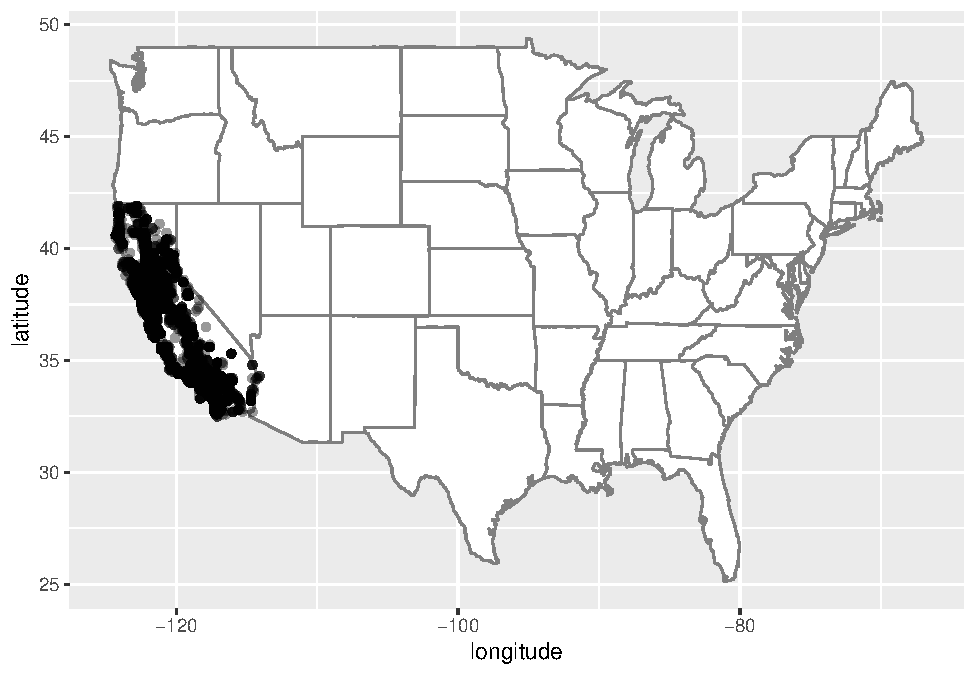
\includegraphics{ACT4114_TP_Part1_Equipe09--1-_files/figure-latex/geolocalisation-1.pdf}

\begin{Shaded}
\begin{Highlighting}[]
\NormalTok{mapCalifornia }\OtherTok{\textless{}{-}} \FunctionTok{borders}\NormalTok{(}\AttributeTok{database =} \StringTok{"county"}\NormalTok{, }\AttributeTok{region =} \StringTok{"california"}\NormalTok{,}
                  \AttributeTok{colour=}\StringTok{"gray50"}\NormalTok{, }\AttributeTok{fill=}\StringTok{"white"}\NormalTok{)}
\FunctionTok{ggplot}\NormalTok{(}\AttributeTok{data =}\NormalTok{ data, }\FunctionTok{aes}\NormalTok{(}\AttributeTok{x =}\NormalTok{ longitude, }\AttributeTok{y =}\NormalTok{ latitude, }\AttributeTok{col=}\NormalTok{ )) }\SpecialCharTok{+}
\NormalTok{    mapCalifornia }\SpecialCharTok{+} \FunctionTok{geom\_point}\NormalTok{(}\AttributeTok{alpha =}\NormalTok{ .}\DecValTok{4}\NormalTok{)  }
\end{Highlighting}
\end{Shaded}

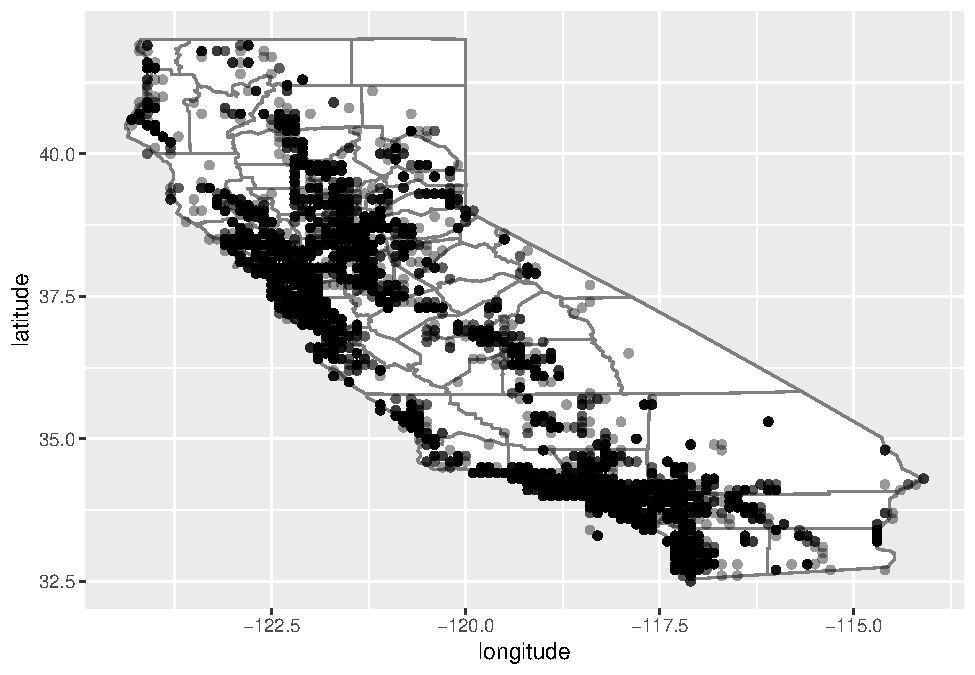
\includegraphics{ACT4114_TP_Part1_Equipe09--1-_files/figure-latex/geolocalisation-2.pdf}

\begin{Shaded}
\begin{Highlighting}[]
\FunctionTok{md.pattern}\NormalTok{(data, }\AttributeTok{rotate.names =}\NormalTok{ T)}
\end{Highlighting}
\end{Shaded}

\begin{verbatim}
##  /\     /\
## {  `---'  }
## {  O   O  }
## ==>  V <==  No need for mice. This data set is completely observed.
##  \  \|/  /
##   `-----'
\end{verbatim}

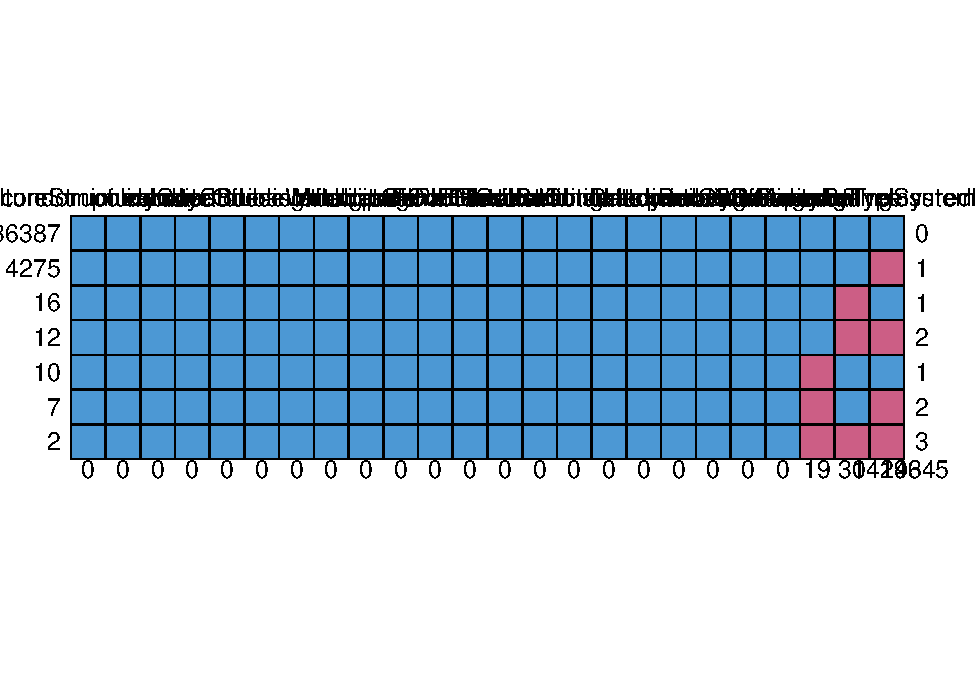
\includegraphics{ACT4114_TP_Part1_Equipe09--1-_files/figure-latex/geolocalisation-3.pdf}

\begin{verbatim}
##       agricultureStructureIndicator condominiumIndicator policyCount countyCode
## 50690                             1                    1           1          1
##                                   0                    0           0          0
##       communityRatingSystemDiscount dateOfLoss elevatedBuildingIndicator
## 50690                             1          1                         1
##                                   0          0                         0
##       houseWorship latitude longitude locationOfContents lowestFloorElevation
## 50690            1        1         1                  1                    1
##                  0        0         0                  0                    0
##       numberOfFloorsInTheInsuredBuilding nonProfitIndicator occupancyType
## 50690                                  1                  1             1
##                                        0                  0             0
##       amountPaidOnBuildingClaim smallBusinessIndicatorBuilding state
## 50690                         1                              1     1
##                               0                              0     0
##       totalBuildingInsuranceCoverage totalContentsInsuranceCoverage
## 50690                              1                              1
##                                    0                              0
##       primaryResidence totalAmount  
## 50690                1           1 0
##                      0           0 0
\end{verbatim}

\hypertarget{explication-des-variables}{%
\subsection{Explication des variables}\label{explication-des-variables}}

\begin{Shaded}
\begin{Highlighting}[]
\CommentTok{\# Changement des noms de variables}

\FunctionTok{colnames}\NormalTok{(data) }\OtherTok{\textless{}{-}} \FunctionTok{c}\NormalTok{(}\StringTok{"EstAgricole"}\NormalTok{,}
                    \StringTok{"EstCondo"}\NormalTok{,}
                    \StringTok{"NbPolice"}\NormalTok{,}
                    \StringTok{"CountyCode"}\NormalTok{,}
                    \StringTok{"TypeRabais"}\NormalTok{,}
                    \StringTok{"DateSiniste"}\NormalTok{,}
                    \StringTok{"EstElevé"}\NormalTok{,}
                    \StringTok{"EstReligieux"}\NormalTok{,}
                    \StringTok{"Latitude"}\NormalTok{,}
                    \StringTok{"Longitude"}\NormalTok{,}
                    \StringTok{"LocContenu"}\NormalTok{,}
                    \StringTok{"ÉlévationPlancher"}\NormalTok{,}
                    \StringTok{"NbÉtage"}\NormalTok{,}
                    \StringTok{"EstNonProfit"}\NormalTok{,}
                    \StringTok{"TypeHabitation"}\NormalTok{,}
                    \StringTok{"ApresFIRM"}\NormalTok{,}
                    \StringTok{"EstPME"}\NormalTok{,}
                    \StringTok{"État"}\NormalTok{,}
                    \StringTok{"CouvertureBatiment"}\NormalTok{,}
                    \StringTok{"CouvertureContenu"}\NormalTok{,}
                    \StringTok{"EstResPrimaire"}\NormalTok{,}
                    \StringTok{"PerteTotal"}\NormalTok{)}


\CommentTok{\# Transformations des variables en classes appropriées}

\NormalTok{data}\SpecialCharTok{$}\NormalTok{EstAgricole }\OtherTok{\textless{}{-}} \FunctionTok{factor}\NormalTok{(data}\SpecialCharTok{$}\NormalTok{EstAgricole)}

\NormalTok{data}\SpecialCharTok{$}\NormalTok{TypeRabais }\OtherTok{\textless{}{-}} \FunctionTok{factor}\NormalTok{(data}\SpecialCharTok{$}\NormalTok{TypeRabais)}

\NormalTok{data}\SpecialCharTok{$}\NormalTok{EstElevé }\OtherTok{\textless{}{-}} \FunctionTok{factor}\NormalTok{(data}\SpecialCharTok{$}\NormalTok{EstElevé)}

\NormalTok{data}\SpecialCharTok{$}\NormalTok{EstReligieux }\OtherTok{\textless{}{-}} \FunctionTok{factor}\NormalTok{(data}\SpecialCharTok{$}\NormalTok{EstReligieux)}

\NormalTok{data}\SpecialCharTok{$}\NormalTok{LocContenu }\OtherTok{\textless{}{-}} \FunctionTok{factor}\NormalTok{(data}\SpecialCharTok{$}\NormalTok{LocContenu)}

\NormalTok{data}\SpecialCharTok{$}\NormalTok{NbÉtage }\OtherTok{\textless{}{-}} \FunctionTok{factor}\NormalTok{(data}\SpecialCharTok{$}\NormalTok{NbÉtage)}

\NormalTok{data}\SpecialCharTok{$}\NormalTok{EstNonProfit }\OtherTok{\textless{}{-}} \FunctionTok{factor}\NormalTok{(data}\SpecialCharTok{$}\NormalTok{EstNonProfit)}

\NormalTok{data}\SpecialCharTok{$}\NormalTok{TypeHabitation }\OtherTok{\textless{}{-}} \FunctionTok{factor}\NormalTok{(data}\SpecialCharTok{$}\NormalTok{TypeHabitation)}

\NormalTok{data}\SpecialCharTok{$}\NormalTok{ApresFIRM }\OtherTok{\textless{}{-}} \FunctionTok{factor}\NormalTok{(data}\SpecialCharTok{$}\NormalTok{ApresFIRM)}

\NormalTok{data}\SpecialCharTok{$}\NormalTok{EstPME }\OtherTok{\textless{}{-}} \FunctionTok{factor}\NormalTok{(data}\SpecialCharTok{$}\NormalTok{EstPME)}

\NormalTok{data}\SpecialCharTok{$}\NormalTok{EstResPrimaire }\OtherTok{\textless{}{-}} \FunctionTok{factor}\NormalTok{(data}\SpecialCharTok{$}\NormalTok{EstResPrimaire)}
\end{Highlighting}
\end{Shaded}

\begin{Shaded}
\begin{Highlighting}[]
\FunctionTok{str}\NormalTok{(data)}
\end{Highlighting}
\end{Shaded}

\begin{verbatim}
## 'data.frame':    50690 obs. of  22 variables:
##  $ EstAgricole       : Factor w/ 2 levels "0","1": 1 1 1 1 1 1 1 1 1 1 ...
##  $ EstCondo          : Factor w/ 2 levels "0","1": 1 1 1 1 1 1 1 1 1 1 ...
##  $ NbPolice          : int  1 1 1 1 1 1 1 1 1 1 ...
##  $ CountyCode        : num  6013 6059 6085 6059 6059 ...
##  $ TypeRabais        : Factor w/ 9 levels "1","2","3","5",..: 9 7 5 9 9 9 1 9 9 5 ...
##  $ DateSiniste       : Date, format: "1995-01-09" "2017-01-22" ...
##  $ EstElevé          : Factor w/ 2 levels "0","1": 1 1 1 1 1 1 1 2 1 1 ...
##  $ EstReligieux      : Factor w/ 2 levels "0","1": 1 1 1 1 1 1 1 1 1 1 ...
##  $ Latitude          : num  37.9 33.9 37.5 33.8 33.4 39.3 38.7 37.6 32.8 38.1 ...
##  $ Longitude         : num  -122 -118 -122 -118 -118 ...
##  $ LocContenu        : Factor w/ 8 levels "0","1","2","3",..: 1 1 1 1 5 1 1 1 1 1 ...
##  $ ÉlévationPlancher : num  0 0 0 0 0 0 0 0 0 0 ...
##  $ NbÉtage           : Factor w/ 6 levels "1","2","3","4",..: 2 1 1 1 2 2 1 2 1 3 ...
##  $ EstNonProfit      : Factor w/ 2 levels "0","1": 1 1 1 1 1 1 1 1 1 1 ...
##  $ TypeHabitation    : Factor w/ 3 levels "1","2","3": 1 1 1 1 1 1 1 1 1 1 ...
##  $ ApresFIRM         : Factor w/ 28511 levels "0","0.66","1",..: 7414 18573 25908 1 17106 1 26615 1 1 5894 ...
##  $ EstPME            : Factor w/ 2 levels "0","1": 1 1 1 1 1 1 1 1 1 1 ...
##  $ État              : chr  "CA" "CA" "CA" "CA" ...
##  $ CouvertureBatiment: int  185000 250000 203500 120000 250000 20000 173700 185000 86400 20000 ...
##  $ CouvertureContenu : int  60000 100000 63000 0 100000 8000 30000 10000 20800 5000 ...
##  $ EstResPrimaire    : Factor w/ 2 levels "0","1": 1 2 2 2 2 2 2 1 1 1 ...
##  $ PerteTotal        : num  0 0 32887 0 0 ...
\end{verbatim}

\begin{Shaded}
\begin{Highlighting}[]
\FunctionTok{summary}\NormalTok{(data)}
\end{Highlighting}
\end{Shaded}

\begin{verbatim}
##  EstAgricole EstCondo     NbPolice         CountyCode     TypeRabais   
##  0:50663     0:49617   Min.   :  1.000   Min.   :6001   10     :21368  
##  1:   27     1: 1073   1st Qu.:  1.000   1st Qu.:6037   7      :13631  
##                        Median :  1.000   Median :6065   6      : 4102  
##                        Mean   :  1.056   Mean   :6063   8      : 3157  
##                        3rd Qu.:  1.000   3rd Qu.:6087   5      : 3090  
##                        Max.   :103.000   Max.   :6115   3      : 1897  
##                                                         (Other): 3445  
##   DateSiniste         EstElevé  EstReligieux    Latitude       Longitude     
##  Min.   :1974-12-14   0:45040   0:50662      Min.   :32.50   Min.   :-124.3  
##  1st Qu.:1986-02-14   1: 5650   1:   28      1st Qu.:34.10   1st Qu.:-122.5  
##  Median :1995-03-10                          Median :37.40   Median :-121.5  
##  Mean   :1995-11-15                          Mean   :36.49   Mean   :-120.6  
##  3rd Qu.:2001-01-11                          3rd Qu.:38.50   3rd Qu.:-118.4  
##  Max.   :2022-03-28                          Max.   :41.90   Max.   :-114.1  
##                                                                              
##    LocContenu    ÉlévationPlancher NbÉtage   EstNonProfit TypeHabitation
##  0      :21152   Min.   : -10.90   1:30199   0:50679      1:40718       
##  3      :18321   1st Qu.:   0.00   2:14954   1:   11      2: 4865       
##  4      : 7862   Median :   0.00   3: 4182                3: 5107       
##  2      : 2544   Mean   :  14.48   4: 1012                              
##  7      :  406   3rd Qu.:   0.00   5:  310                              
##  6      :  246   Max.   :9992.00   6:   33                              
##  (Other):  159                                                          
##    ApresFIRM     EstPME        État           CouvertureBatiment
##  0      :18919   0:50510   Length:50690       Min.   :       0  
##  750    :  260   1:  180   Class :character   1st Qu.:   35000  
##  35000  :  147             Mode  :character   Median :  100000  
##  10000  :   86                                Mean   :  125051  
##  250000 :   84                                3rd Qu.:  185000  
##  500    :   76                                Max.   :22656800  
##  (Other):31118                                                  
##  CouvertureContenu EstResPrimaire   PerteTotal    
##  Min.   :     0    0:36070        Min.   :     0  
##  1st Qu.:     0    1:14620        1st Qu.:     0  
##  Median :  5000                   Median :     0  
##  Mean   : 23029                   Mean   :  1858  
##  3rd Qu.: 30000                   3rd Qu.:     1  
##  Max.   :500000                   Max.   :500000  
## 
\end{verbatim}

\begin{Shaded}
\begin{Highlighting}[]
\NormalTok{data }\OtherTok{\textless{}{-}} \FunctionTok{subset}\NormalTok{(data, data}\SpecialCharTok{$}\NormalTok{PerteTotal }\SpecialCharTok{\textgreater{}} \DecValTok{1}\NormalTok{)}
\FunctionTok{table}\NormalTok{(data}\SpecialCharTok{$}\NormalTok{EstPME)}
\end{Highlighting}
\end{Shaded}

\begin{verbatim}
## 
##     0     1 
## 10351    77
\end{verbatim}

\begin{Shaded}
\begin{Highlighting}[]
\CommentTok{\#Changement d\textquotesingle{}echelle, log}
\FunctionTok{ggplot}\NormalTok{(}\AttributeTok{data =}\NormalTok{ data, }\FunctionTok{aes}\NormalTok{(}\AttributeTok{x =}\NormalTok{ EstAgricole, }\AttributeTok{y =} \FunctionTok{log}\NormalTok{(PerteTotal) ))}\SpecialCharTok{+}
  \FunctionTok{geom\_boxplot}\NormalTok{()}
\end{Highlighting}
\end{Shaded}

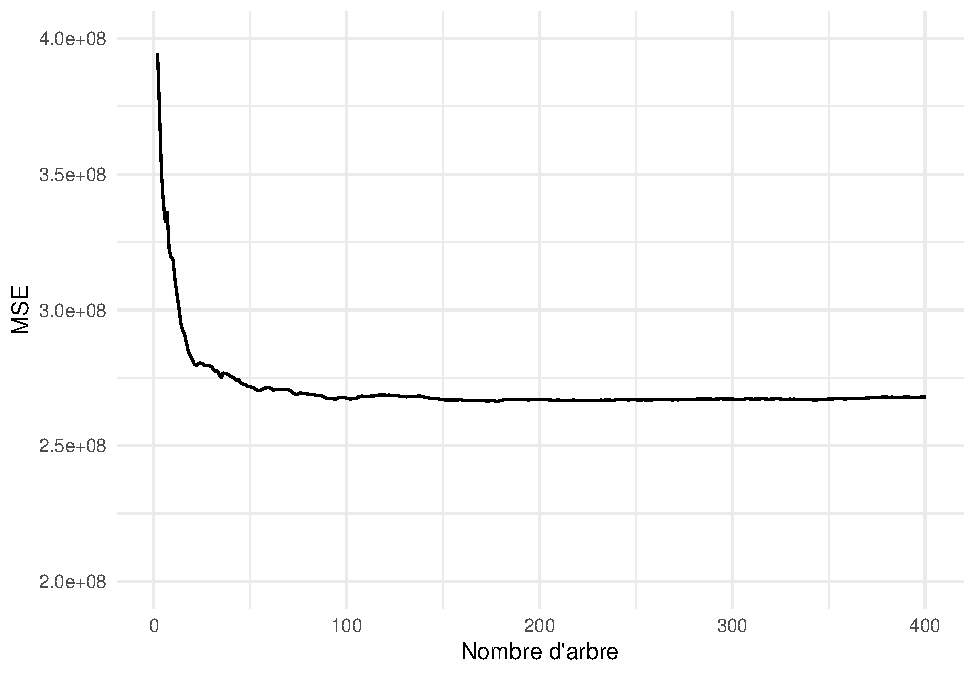
\includegraphics{ACT4114_TP_Part1_Equipe09--1-_files/figure-latex/unnamed-chunk-2-1.pdf}

\begin{Shaded}
\begin{Highlighting}[]
\CommentTok{\#Changement d\textquotesingle{}echelle, log}
\FunctionTok{ggplot}\NormalTok{(}\AttributeTok{data =}\NormalTok{ data, }\FunctionTok{aes}\NormalTok{(}\AttributeTok{x =}\NormalTok{ EstPME, }\AttributeTok{y =} \FunctionTok{log}\NormalTok{(PerteTotal) ))}\SpecialCharTok{+}
  \FunctionTok{geom\_boxplot}\NormalTok{()}
\end{Highlighting}
\end{Shaded}

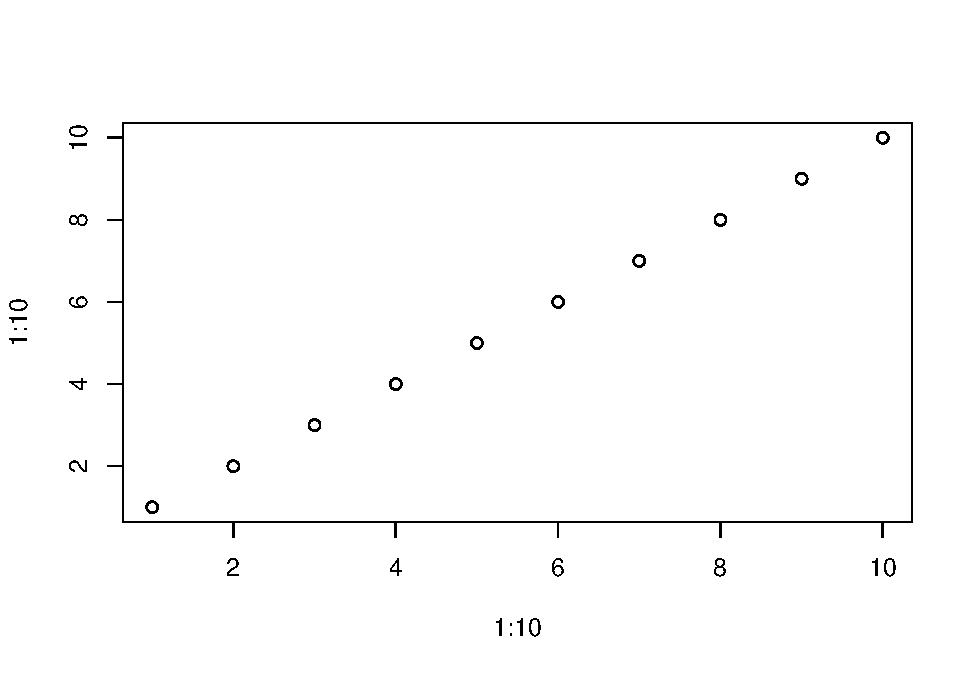
\includegraphics{ACT4114_TP_Part1_Equipe09--1-_files/figure-latex/unnamed-chunk-2-2.pdf}

\begin{Shaded}
\begin{Highlighting}[]
\FunctionTok{ggplot}\NormalTok{(}\AttributeTok{data =}\NormalTok{ data, }\FunctionTok{aes}\NormalTok{(}\AttributeTok{x =}\NormalTok{ NbPolice, }\AttributeTok{y =}\NormalTok{ PerteTotal ))}\SpecialCharTok{+}
  \FunctionTok{geom\_point}\NormalTok{()}
\end{Highlighting}
\end{Shaded}

\includegraphics{ACT4114_TP_Part1_Equipe09--1-_files/figure-latex/unnamed-chunk-2-3.pdf}

\begin{Shaded}
\begin{Highlighting}[]
\FunctionTok{ggplot}\NormalTok{(}\AttributeTok{data =}\NormalTok{ data, }\FunctionTok{aes}\NormalTok{(}\AttributeTok{x =}\NormalTok{ TypeRabais, }\AttributeTok{y =} \FunctionTok{log}\NormalTok{(PerteTotal) ))}\SpecialCharTok{+}
  \FunctionTok{geom\_boxplot}\NormalTok{()}
\end{Highlighting}
\end{Shaded}

\includegraphics{ACT4114_TP_Part1_Equipe09--1-_files/figure-latex/unnamed-chunk-2-4.pdf}

\newpage

\hypertarget{conclusion}{%
\section{Conclusion}\label{conclusion}}

\newpage

\hypertarget{bibliographie}{%
\section{Bibliographie}\label{bibliographie}}

\newpage

\hypertarget{annexe}{%
\section{Annexe}\label{annexe}}

\end{document}
